\documentclass[border=4pt]{standalone}
\usepackage[utf8]{inputenc}\usepackage[T1]{fontenc}\usepackage{mathptmx}
\usepackage{tikz}\usetikzlibrary{positioning,arrows.meta,calc,fit}
\begin{document}
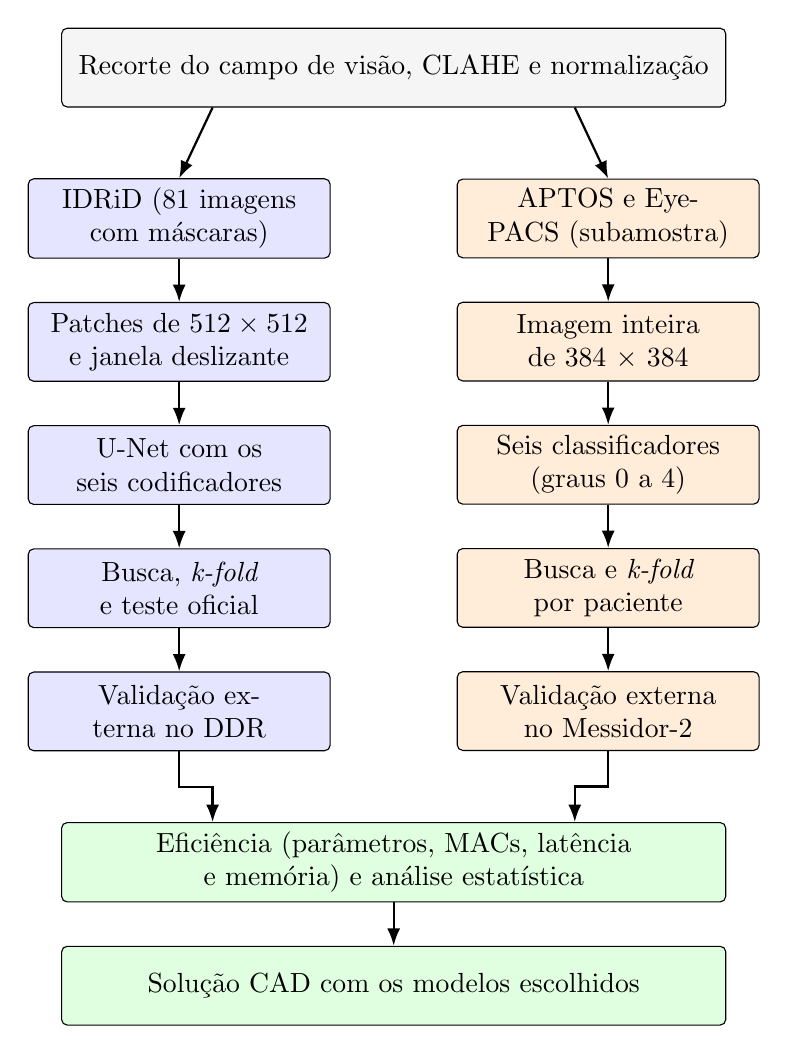
\begin{tikzpicture}[font=\normalsize,node distance=0.55cm and 0.6cm,
  b/.style={draw,rounded corners=2pt,align=center,text width=3.6cm,minimum height=1.0cm,fill=#1},b/.default=gray!8,
  arr/.style={-{Latex[length=2.2mm]},thick}]
\node[b=blue!10] (s1) {IDRiD (81 imagens com máscaras)};
\node[b=blue!10,below=of s1] (s2) {Patches de $512\times512$ e janela deslizante};
\node[b=blue!10,below=of s2] (s3) {U-Net com os seis codificadores};
\node[b=blue!10,below=of s3] (s4) {Busca, \textit{k-fold} e teste oficial};
\node[b=blue!10,below=of s4] (s5) {Validação externa no DDR};
\node[b=orange!15,right=1.6cm of s1] (c1) {APTOS e EyePACS (subamostra)};
\node[b=orange!15,below=of c1] (c2) {Imagem inteira de $384\times384$};
\node[b=orange!15,below=of c2] (c3) {Seis classificadores (graus 0 a 4)};
\node[b=orange!15,below=of c3] (c4) {Busca e \textit{k-fold} por paciente};
\node[b=orange!15,below=of c4] (c5) {Validação externa no Messidor-2};
\node[b,above=0.9cm of $(s1.north)!0.5!(c1.north)$,text width=8.2cm] (p) {Recorte do campo de visão, CLAHE e normalização};
\node[b=green!12,below=0.9cm of $(s5.south)!0.5!(c5.south)$,text width=8.2cm] (e) {Eficiência (parâmetros, MACs, latência e memória) e análise estatística};
\node[b=green!12,below=of e,text width=8.2cm] (cad) {Solução CAD com os modelos escolhidos};
\foreach \i/\j in {1/2,2/3,3/4,4/5}{\draw[arr] (s\i)--(s\j); \draw[arr] (c\i)--(c\j);}
\draw[arr] (p.south) ++(-2.3,0) -- (s1.north); \draw[arr] (p.south) ++(2.3,0) -- (c1.north);
\draw[arr] (s5.south) -- ++(0,-0.45) -| ([xshift=-2.3cm]e.north);
\draw[arr] (c5.south) -- ++(0,-0.45) -| ([xshift=2.3cm]e.north);
\draw[arr] (e)--(cad);
\end{tikzpicture}
\end{document}
